%!TEX root = ../report.tex
\documentclass[../report.tex]{subfiles}

\begin{document}
    \section{Evaluation}
    \label{sec:evaluation}

    % **Experiment 1:** Train a model from scratch and compare it with a pre-trained model using synthetic data and the real UAVid dataset. 

    % **Experiment 2:** Train the model exclusively on the real dataset, and then use that model as a basis to train on synthetic data to evaluate transfer capabilities.
    
    % **Experiment 3:** Train on synthetic data and test the model performance using the real dataset to analyze how well synthetic training translates to real-world conditions.
    
    % **Experiment 4:** Investigate the impact of training on data collected at different heights to determine if this variation leads to performance improvements. 
    
    % **Experiment 5:** Train using datasets collected at combined heights to see if this approach enhances the model’s capabilities compared to using singular height datasets.
    
    % **Experiment 6:** Experiment with different dataset sizes.
    % % beginning with 200 synthetic images and progressively adding sets of 200 more. The goal here is to assess whether increasing the dataset size enhances the performance of semantic segmentation. 

    \subsection{Experimental Setup}
    \subsubsection{Datasets}
    Evaluation of semantic segmentation is done using real-world and synthetic aerial imagery datasets. Our primary real-world data source is the UAVid dataset, consisting of 300 high-resolution (3840×2160 pixels) aerial images with train, val, and test split of 3:1:2 captured from a 50-meter altitude. This dataset showcases urban environments with diverse architectural styles. To complement the real-world data, we generated synthetic datasets using various environments from UE. The City Park environment, our largest synthetic dataset, contains over 1,200 images featuring diverse urban park scenery with multiple vegetation types and building structures. The Modular Downtown West environment provides 500 images of dense urban settings, while the Neighborhood environment contributes 300 images of residential areas with varied street layouts and building arrangements. Additionally, incorporated the Landscape Mountain's Village environment to capture snow-covered scenery. To maintain balanced comparisons with UAVid, randomly sampled 300 images from each synthetic environment. As mentioned in the earlier sections, a unique aspect of synthetic data collection involves capturing images from three distinct altitudes: 10 meters, 15 meters, and 25 meters. This approach effectively triples (10m, 15m, 25m) the total number of images collected per environment, ensuring a diverse range of perspectives. Cross-dataset performance is analyzed by evaluating synthetic-to-real and real-to-synthetic dataset transfer capabilities.
    
    \subsubsection{Training Configuration}
    
    Evaluated two model architectures: UNet with a ResNet34 backbone (pretrained on ImageNet, $\sim\text{24M}$ parameters) and SegFormer-B3 (a hierarchical transformer pretrained on ImageNet and Cityscapes, $\sim\text{47M}$ parameters). Initially, trained for 100 epochs to observe the training progress and found that the validation loss was getting higher than the training loss leading to overfitting and performance plateaued beyond 60 epochs. 
    
    As a result, we adjusted our training duration to 60 epochs for all future experiments. A batch size of 16 is set to meet the hardware constraints and the memory requirements of the SegFormer-B3 model. These configurations, along with the hyperparameters outlined in the Methodology section, are consistently maintained across all experiments to ensure uniformity and reliability in the training process. 

    \subsection{Pixel Distribution in Synthetic and Real Datasets}
    Figure~\ref{fig:pixel_analysis} illustrates the class-wise pixel distribution, with darker bars representing the synthetic \textit{City Park} dataset and lighter bars indicating the \textit{UAVid}'s pixel count in percentage.
    
    The difference in building class representation between UAVid (28\%) and synthetic data (3\%) illustrates how a City Park environment leads to a higher dominance of trees and clutter in pixel distribution. This shows that the choice of synthetic environment significantly affects class distributions and might not be aligned with real-world scenarios. 

    Each synthetic environment reflects its specific characteristics, for example: a \textit{Neighborhood Pack} will emphasize structured buildings, while a \textit{City Park} will highlight trees and vegetation. This variation highlights the need to select environments carefully to ensure they accurately represent the complexities of real-world scenes for effective data application.

    \begin{figure}[h]
        \centering
        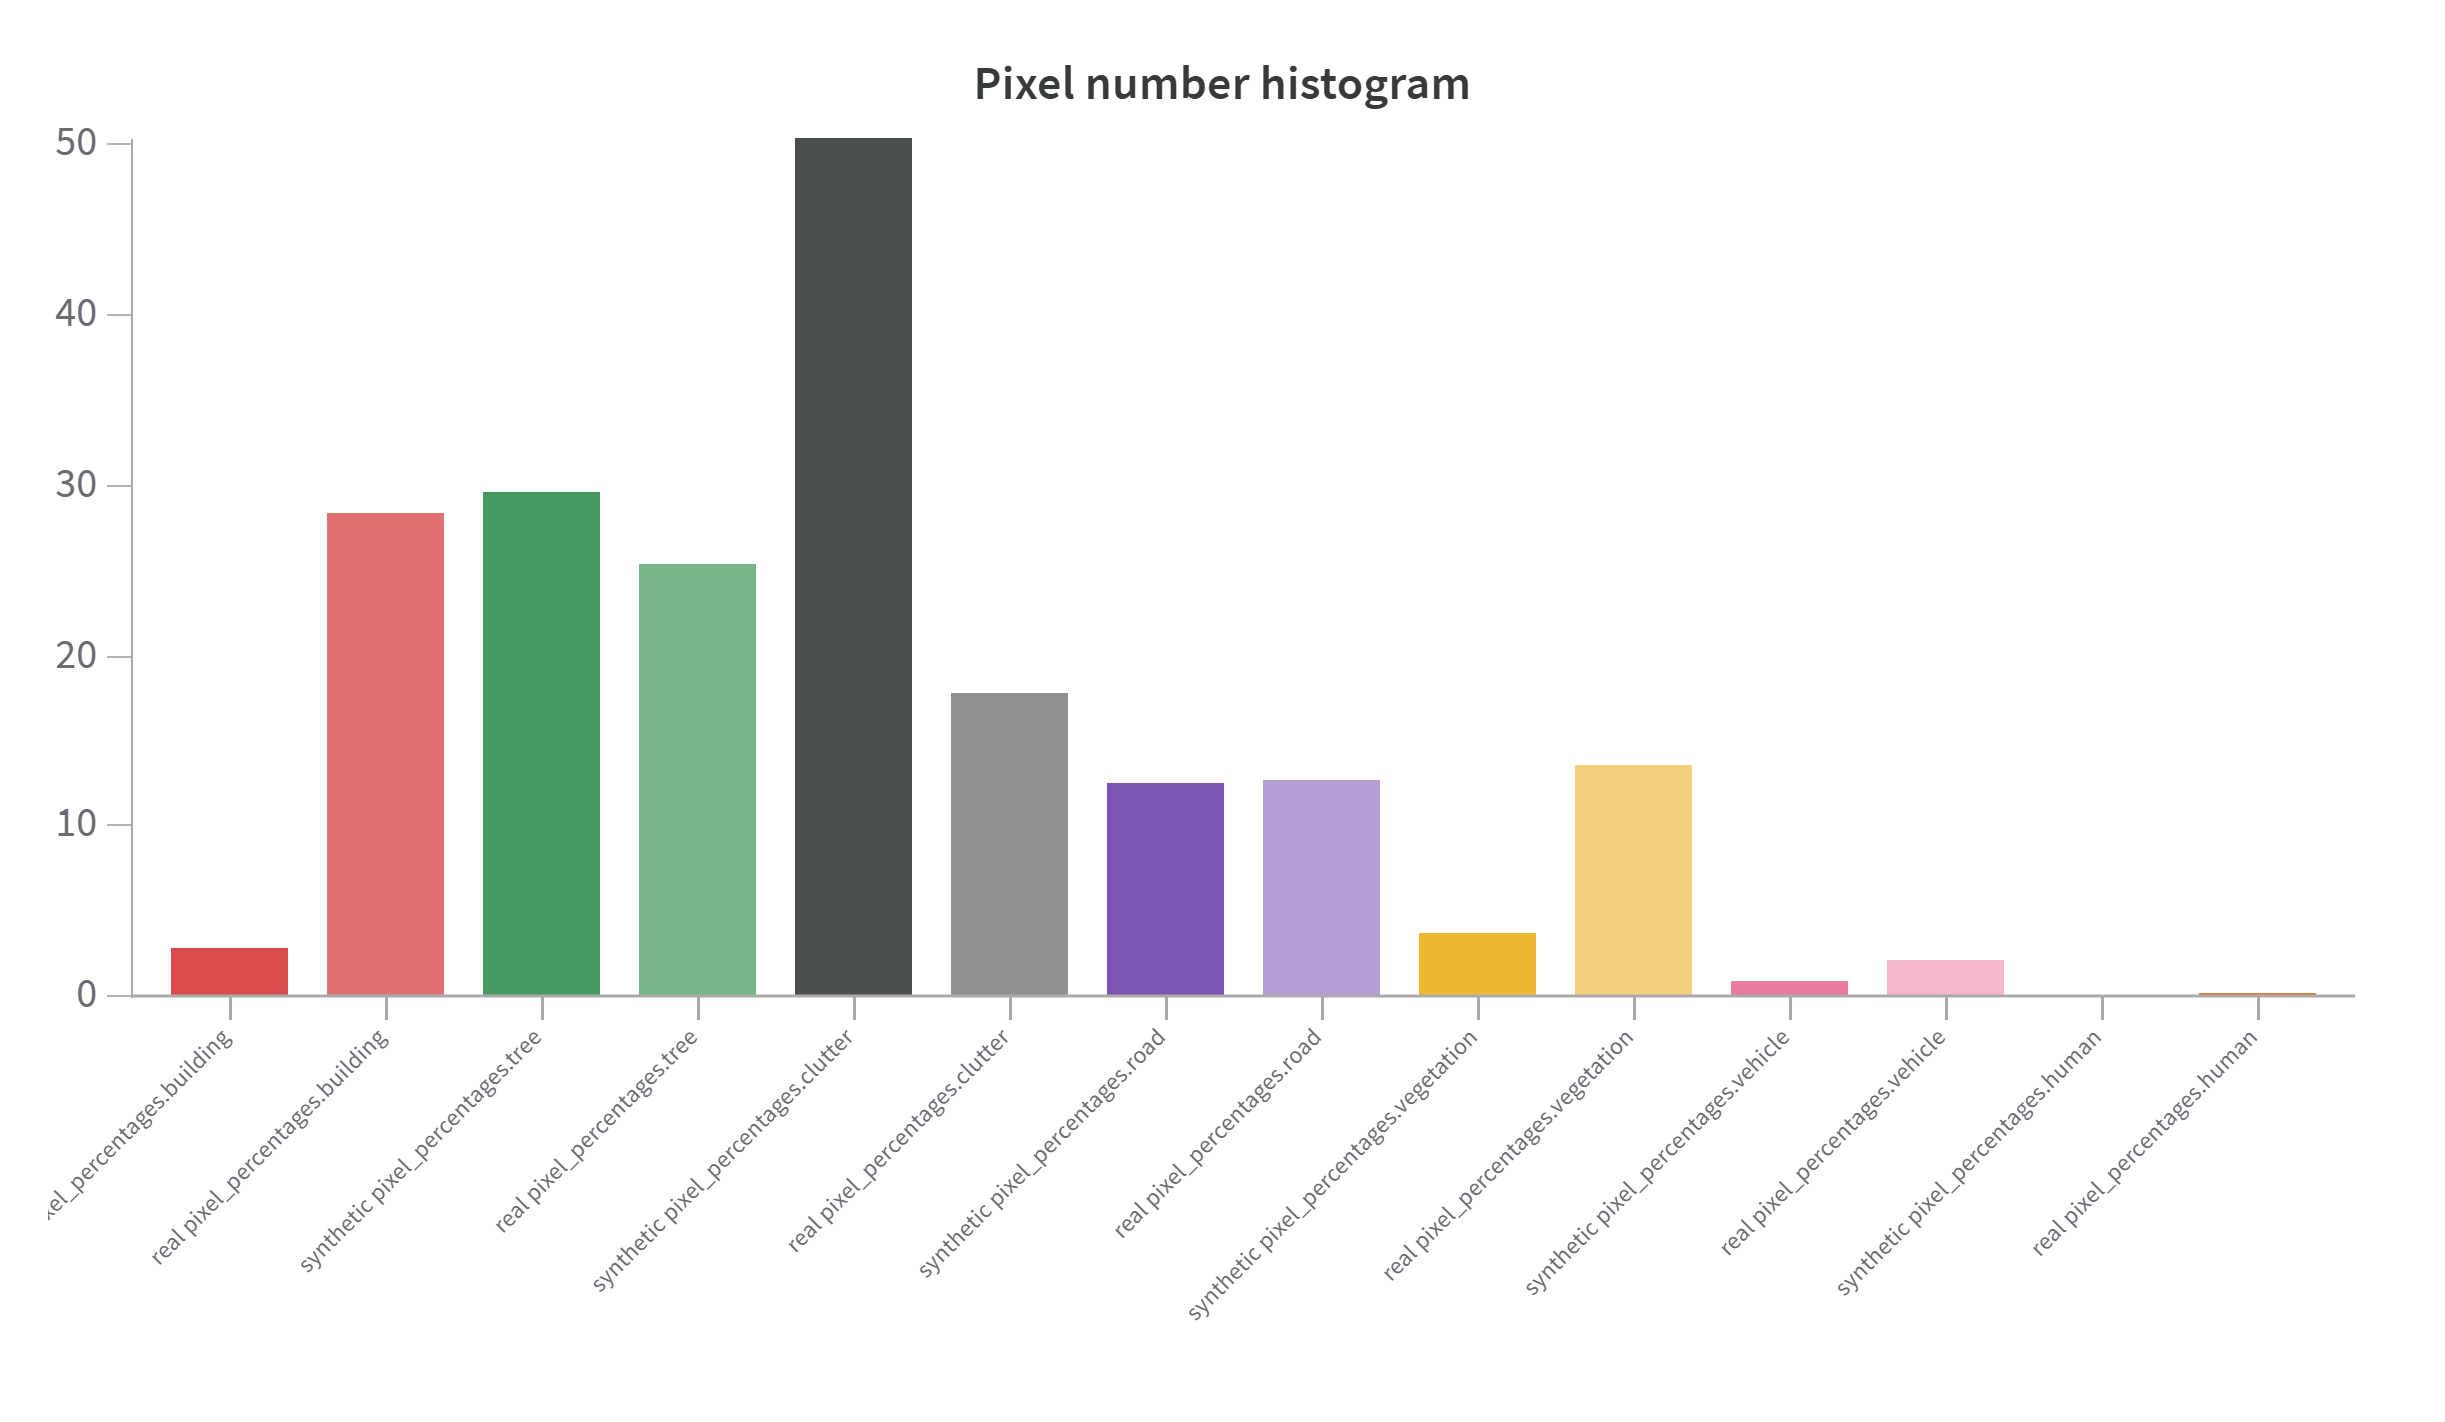
\includegraphics[width=0.9\linewidth]{figures/pixel_analysis.png}
        \caption{Pixel-Class Distribution: synthetic and real dataset's classes building(red), tree(green), clutter(black), road(purple), vegetation(yellow), vehicle(pink), human(orange).}
        \label{fig:pixel_analysis}
    \end{figure}
    
    
\end{document}
